
\section{NetConfigQA 2.0: 벤치마크 데이터셋}
\subsection{토폴로지 설계}
기본 토폴로지(Lab-A)는 10대의 Cisco IOS 라우터로 구성된 Service Provider MPLS VPN 네트워크이다. P(Provider) 라우터 4대, PE(Provider Edge) 라우터 2대, Leaf 스위치 4대가 OSPF, MP-BGP, LDP, VRF 구성으로 연결되어 있다. 파이프라인의 확장성을 검증하기 위해 National Converged Network(NCN) 시리즈를 설계하였다. 동일한 파이프라인과 정책 파일(\texttt{policies.json})을 사용하면서 토폴로지만 교체하여, 설정 복잡도의 증가에 따른 데이터셋 자동 확장을 입증한다.

\begin{table*}[!t]
  \caption{토폴로지 요약}
  \label{tab:topology-summary}
  \centering
  \small
  \begin{tabular}{|L{1.6cm}|C{1.2cm}|L{3.0cm}|L{4.2cm}|C{1.8cm}|}
    \hline
    \textbf{Lab} & \textbf{노드} & \textbf{컨셉}    & \textbf{핵심 프로토콜}               & \textbf{QA 수}  \\
    \hline
    Lab-A        & 10          & SP MPLS VPN    & OSPF, BGP, LDP, VRF            & \textbf{1,264} \\
    \hline
    Lab-B        & 20          & NCN 기본 SP      & + NTP, SNMP, AAA, Banner       & \textbf{2,154} \\
    \hline
    Lab-C        & 30          & NCN 보안 + L2VPN & + L2VPN, ACL, eBGP, HSRP       & \textbf{2,673} \\
    \hline
    Lab-D        & 40          & NCN 멀티 AS 복합   & + QoS, NetFlow, 3-AS, Waypoint & \textbf{3,371} \\
    \hline
    \textbf{합계}  & --          & --             & --                             & \textbf{9,462} \\
    \hline
  \end{tabular}
\end{table*}

모든 설정 파일은 PNETLab 에뮬레이션 환경에서 배포 및 검증되었다. Lab-B\textasciitilde D의 설정은 YAML 토폴로지 정의와 Jinja2 템플릿 기반 Config Generator로 자동 생성하였으며, OSPF/BGP/LDP 프로토콜 수렴을 확인하였다.

\subsection{이중 경로(Dual-Path) QA 생성 파이프라인}
NetConfigQA 2.0은 두 가지 경로로 QA 쌍을 생성한다.

\textbf{경로 A (L1\textasciitilde L3, 규칙 기반):} 설정 파일을 Batfish~\cite{ref17}가 파싱하여 정적 팩트(Static Facts) JSON을 생성한다. \texttt{policies.json}에 정의된 127개 메트릭은 네트워크 운영자가 토폴로지에 대해 일상적으로 확인하는 항목(인터페이스 상태, 라우팅 이웃, ACL 규칙 등)을 Cisco IOS 운영 매뉴얼과 Batfish가 지원하는 분석 범위를 기준으로 체계화한 것이다. 각 메트릭에 대해 질문 템플릿, 스코프 확장 규칙, 답변 타입이 지정되어 있다. 스코프 확장(Scope Expansion) 메커니즘은 12가지 스코프 타입(GLOBAL, DEVICE, DEVICE\_PAIR, AS, OSPF\_AREA, VRF, FLOW 등)에 걸쳐 질문 인스턴스를 동적으로 생성한다. 이 과정에서 하나의 메트릭이 토폴로지 내 모든 해당 엔티티에 대해 자동으로 인스턴스화되므로, 노드 수 증가에 비례하여 QA가 확장된다.

템플릿 기반 생성에서 질문 형태의 단조로움은 스코프 확장 메커니즘(장비명, VRF명, 인터페이스명의 동적 치환)과, L4/L5의 조합적 노드 쌍 샘플링을 통해 완화된다. 후자는 키워드 오버피팅이 아닌 토폴로지 구조 이해를 정답 도출의 전제 조건으로 만든다.

\textbf{경로 B (L4\textasciitilde L5, 절차적):} Batfish 시뮬레이션 엔진을 활용한다. L4에서는 노드 쌍을 샘플링하여 \texttt{traceroute}와 \texttt{reachability} 쿼리를 실행하고, L5에서는 \texttt{fork\_snapshot}으로 지정된 링크/노드를 비활성화한 가상 네트워크 복사본을 생성한 뒤 \texttt{differentialReachability} 쿼리로 장애 영향을 분석한다. 시뮬레이션 결과가 자연어 질문-답변 쌍으로 자동 변환된다.

\begin{figure*}[!t]
  \centering
  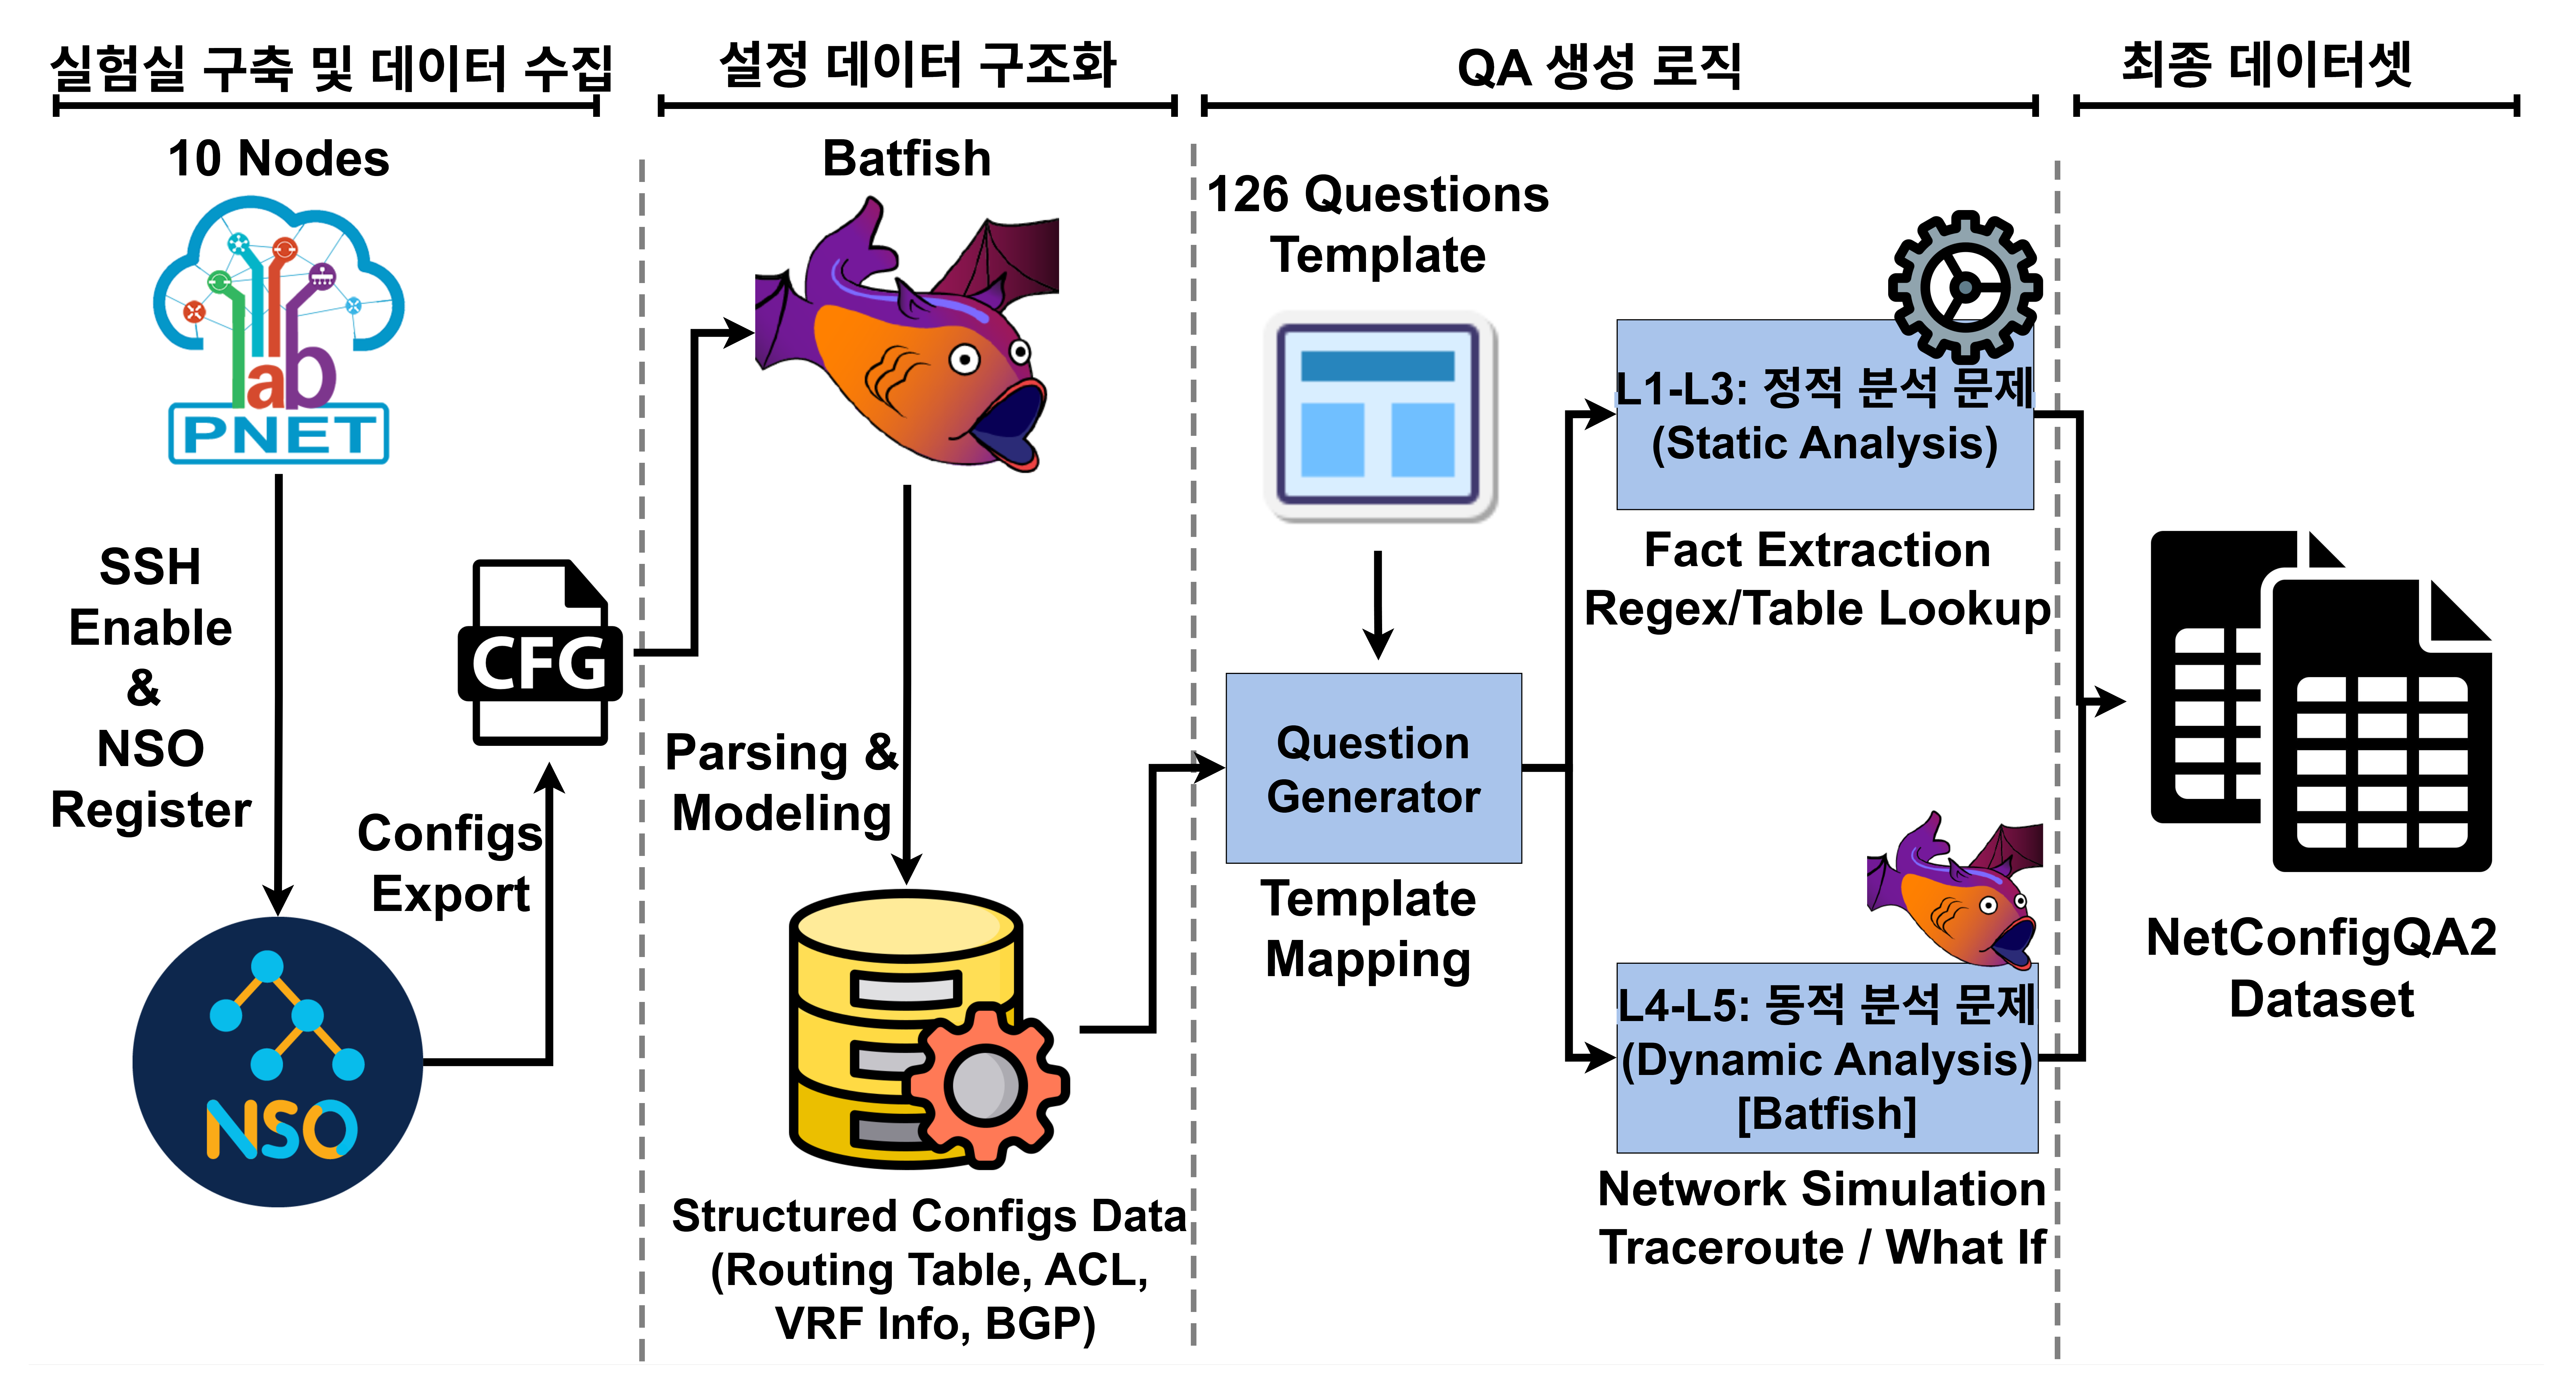
\includegraphics[width=0.8\textwidth]{figure/Pipeline.png}
  \caption{NetConfigQA 2.0 이중 경로 QA 생성 파이프라인. 경로~A는 Batfish 파싱 $\rightarrow$ 정적 팩트 $\rightarrow$ 규칙 기반 생성(L1\textasciitilde L3), 경로~B는 Batfish 시뮬레이션 $\rightarrow$ traceroute/fork\_snapshot $\rightarrow$ 절차적 생성(L4\textasciitilde L5).}
  \label{fig:pipeline}
\end{figure*}

\subsection{5단계 인지 난이도 체계}
Table~\ref{tab:difficulty-taxonomy}은 네트워크 운영자의 인지 부하(Cognitive Load)를 기준으로 설계한 5단계 난이도 체계이다. L1\textasciitilde L3는 설정 파일의 텍스트에서 직접 답을 도출할 수 있는 정적 분석 영역이며, L4\textasciitilde L5는 설정에 필요한 정보가 모두 포함되어 있으나 그래프 알고리즘(OSPF SPF 등)의 실행이 요구되는 동작 추론 영역이다.

\begin{table*}[!t]
  \caption{인지 난이도 체계}
  \label{tab:difficulty-taxonomy}
  \centering
  \small
  \begin{tabular}{|C{1.0cm}|L{2.2cm}|L{3.0cm}|L{3.0cm}|C{2.4cm}|}
    \hline
    \textbf{레벨} & \textbf{인지 활동} & \textbf{질문 본질}  & \textbf{정답 생성 방식}     & \textbf{참조 장비 수} \\
    \hline
    L1          & 사실 추출          & 설정에 무엇이 적혀 있는가? & Config 파싱             & $O(1)$           \\
    \hline
    L2          & 통계 집계          & 네트워크 전체 통계는?    & 전체 장비 순회              & $O(N)$           \\
    \hline
    L3          & 정합성 비교         & 설정 간 논리적 모순은?   & 장비 간 교차 검증            & $O(N^2)$         \\
    \hline
    L4          & 경로 시뮬레이션       & 패킷이 실제로 도착하는가?  & Batfish traceroute    & 프로토콜 시뮬레이션       \\
    \hline
    L5          & 장애 영향 추론       & 장애 시 어떻게 되는가?   & fork\_snapshot + diff & 복수 시뮬레이션         \\
    \hline
  \end{tabular}
\end{table*}

Lab-A의 레벨별 분포와 4개 Lab의 비교는 Table~\ref{tab:level-distribution}에 제시한다. L1은 장비 단위 메트릭(hostname, 인터페이스 IP 등)으로 구성되어 메트릭 수가 고정되므로, Lab-B 이후에서는 새 프로토콜이 추가되어도 L1 질문 수가 일정하다. 반면 L4는 노드 쌍 조합이 $O(N^2)$로 증가하므로 146(Lab-A) $\rightarrow$ 1,657(Lab-D)로 급증하며, 파이프라인이 토폴로지 복잡도에 자동으로 적응함을 보여준다. L2는 GLOBAL 스코프 메트릭(``전체 장비 중 SSH 활성화 비율'')으로 구성되어 노드 수에 관계없이 일정하며, 프로토콜 종류 변화에 따라 소폭 감소한다.

\begin{table*}[!t]
  \caption{Lab별 레벨 분포}
  \label{tab:level-distribution}
  \centering
  \small
  \begin{tabular}{|C{1.1cm}|C{2.3cm}|C{1.6cm}|C{1.6cm}|C{1.6cm}|}
    \hline
    \textbf{레벨} & \textbf{Lab-A} & \textbf{Lab-B} & \textbf{Lab-C} & \textbf{Lab-D} \\
    \hline
    L1          & 660 (52.2\%)   & 1,230          & 1,230          & 1,230          \\
    \hline
    L2          & 104 (8.2\%)    & 101            & 80             & 69             \\
    \hline
    L3          & 252 (19.9\%)   & 255            & 255            & 253            \\
    \hline
    L4          & 146 (11.6\%)   & 441            & 954            & 1,657          \\
    \hline
    L5          & 102 (8.1\%)    & 127            & 154            & 162            \\
    \hline
    \textbf{합계} & \textbf{1,264} & \textbf{2,154} & \textbf{2,673} & \textbf{3,371} \\
    \hline
  \end{tabular}
\end{table*}

\subsection{Type-Aware Accuracy (TA-Acc)}
전통적 NLP 지표는 네트워크 구성 평가에 부적합하다. BERTScore는 의미적으로 다른 IP 주소(\texttt{10.0.1.1}과 \texttt{10.0.1.10})에 0.9 이상의 유사도를 부여하여 모델 간 차이를 변별하지 못한다. Exact Match는 집합의 순서 차이(\texttt{\{r1, r2\}} vs \texttt{\{r2, r1\}})를 오답으로 처리한다. Token F1은 경로의 순서를 무시하여 역방향 경로(\texttt{PE1$\rightarrow$P1$\rightarrow$R1}과 \texttt{R1$\rightarrow$P1$\rightarrow$PE1})를 정답으로 인정한다.

TA-Acc는 각 질문의 답변 타입 $t_i$에 따라 적합한 비교 함수 $f_{t_i}$를 선택하여 개별 점수를 산출하고, 전체 데이터셋에 대해 산술 평균을 취한다.

\textbf{정의.} 데이터셋 $D = \{(q_i, g_i, t_i)\}_{i=1}^{N}$이 주어지고, 모델의 예측을 $p_i$라 할 때, TA-Acc는 다음과 같이 정의된다:
\begin{equation}
  \text{TA-Acc}(D) = \frac{1}{N} \sum_{i=1}^{N} f_{t_i}(\hat{p}_i, \hat{g}_i)
  \label{eq:taacc}
\end{equation}
여기서 $\hat{p}_i$와 $\hat{g}_i$는 각각 예측과 정답에 정규화(소문자 변환, CIDR 표기 제거, 널 값 통합 등)를 적용한 결과이다. 비교 함수 $f_t$는 Table~\ref{tab:taacc-types}에 정의된 6가지 타입별로 다르게 적용된다.

\begin{table}[!t]
  \caption{TA-Acc의 답변 타입별 비교 함수}
  \label{tab:taacc-types}
  \centering
  \small
  \begin{tabular}{|L{1.6cm}|L{2.2cm}|L{3.3cm}|}
    \hline
    \textbf{답변 타입}   & \textbf{비교 함수 $f_t$} & \textbf{적용 예시}      \\
    \hline
    \texttt{set}     & Set F1 (순서 무관)       & BGP 이웃 목록, 인터페이스 집합 \\
    \hline
    \texttt{text}    & 정규화 후 EM             & 호스트네임, IP 주소        \\
    \hline
    \texttt{path}    & Ordered EM           & traceroute 경로       \\
    \hline
    \texttt{number}  & 숫자 추출 후 EM           & 홉 수, AS 번호, 카운트     \\
    \hline
    \texttt{boolean} & 의미 정규화 비교            & SSH 활성화 여부          \\
    \hline
    \texttt{map}     & Key-Value F1         & 장비별 통계 비교           \\
    \hline
  \end{tabular}
\end{table}

\texttt{set}과 \texttt{map} 타입은 F1 Score를 사용하여 0과 1 사이의 연속 점수를 반환한다. 구체적으로, 예측 집합 $P$와 정답 집합 $G$에 대해:
\begin{equation}
  f_{\texttt{set}}(P, G) = \frac{2 \cdot |P \cap G|}{|P| + |G|}
  \label{eq:set-f1}
\end{equation}
\texttt{map} 타입은 (키, 정규화된 값) 쌍을 집합 원소로 취급하여 동일한 F1을 적용한다. 나머지 4개 타입(\texttt{text}, \texttt{path}, \texttt{number}, \texttt{boolean})은 이진 점수(0 또는 1)를 반환하되, 각 타입에 특화된 정규화를 수행한다. 특히 \texttt{path} 타입은 노드 순서를 보존하는 Ordered Exact Match를 적용하여, \texttt{R1$\rightarrow$P1$\rightarrow$PE1}과 \texttt{PE1$\rightarrow$P1$\rightarrow$R1}을 구분한다.

의도적으로 Token F1 fallback을 배제하였다. 네트워크 데이터에서 Token F1은 부분 일치에 과도한 점수를 부여하여(예: 경로의 일부 노드만 맞춰도 높은 점수), 모델 간 변별력을 저하시키기 때문이다.

\textbf{집계 방식.} 전체 QA에 대한 산술 평균(Micro Average)을 기본 지표로 사용하되, 레벨별 분포 불균형의 영향을 통제하기 위해 Level-Macro Average를 병행 보고한다. Level-Macro Average는 각 레벨의 TA-Acc를 먼저 산출한 뒤 5개 레벨의 산술 평균을 취한 것으로, L4 질문이 지배적인 대규모 토폴로지에서 Micro Average와의 괴리를 확인하는 데 유용하다.

\subsection{Ground Truth 검증}
Ground Truth는 Batfish~\cite{ref17}의 formal network analysis로 정의된다. Batfish는 설정 파일로부터 결정적(deterministic) 계산을 수행하는 네트워크 시뮬레이터로, Header Space Analysis~\cite{ref22}, VeriFlow~\cite{ref23}, Minesweeper~\cite{ref24} 등과 함께 네트워크 정형 검증 분야의 핵심 도구이다. NetConfEval~\cite{ref5}에서도 oracle로 사용된 바 있으며, Config2Spec~\cite{ref20}과 DNA~\cite{ref25}는 Batfish 위에서 설정 명세 추출 및 차등 분석을 수행하며, Campion~\cite{ref29}은 라우터 설정 쌍의 동작 차이를 자동 디버깅한다. Brown et al.~\cite{ref32}은 Batfish가 연구 프로토타입에서 산업용 도구로 진화한 과정을 정리하며, 설정 분석 도구의 신뢰성을 뒷받침한다. 파이프라인 정확성 검증을 위해 3가지 독립적 방법을 사용한다.

\textbf{Method 1 (독립 구문 분석기):} Batfish를 사용하지 않는 Python+Regex 기반 파서(약 2,100줄)가 설정 파일에서 L1\textasciitilde L3 정답을 독립적으로 재도출한다. 4개 Lab에서 총 5,719건을 전수 검증하였다.

\begin{table}[!t]
  \caption{Ground Truth 검증 결과. ``전체 일치율''은 시뮬레이션 의존 메트릭을 포함한 수치이며, ``정적 검증 범위''는 이를 제외하고 독립 파서로 검증 가능한 범위만의 일치율이다.}
  \label{tab:gt-validation}
  \centering
  \small
  \begin{tabular}{|L{2.1cm}|C{1.2cm}|C{1.2cm}|C{1.5cm}|}
    \hline
    \textbf{Lab}  & \textbf{검증 건수} & \textbf{전체 일치율} & \textbf{정적 검증 범위} \\
    \hline
    Lab-A (10 노드) & 1,016          & 99.9\%          & \textbf{99.9\%}   \\
    \hline
    Lab-B (20 노드) & 1,586          & 92.3\%          & \textbf{99.1\%}   \\
    \hline
    Lab-C (30 노드) & 1,565          & 92.8\%          & \textbf{98.2\%}   \\
    \hline
    Lab-D (40 노드) & 1,552          & 92.5\%          & \textbf{98.4\%}   \\
    \hline
  \end{tabular}
\end{table}

``전체 일치율''이 Lab-B\textasciitilde D에서 92\%대인 것은 GT 오류가 아니라 \emph{독립 파서의 검증 범위 한계}에 기인한다. 시뮬레이션 의존 메트릭(L4/L5 traceroute 결과 등)은 Python+Regex 파서로 재도출이 원리적으로 불가능하여 불일치로 집계되지만, 이는 Method~3(PNETLab CLI)에서 별도로 검증한다. 불일치 원인을 분류하면 시뮬레이션 의존(57\%), Batfish 파싱 한계(37\%), 독립 파서 한계(6\%)이며, 정적 팩트의 실질 불일치는 4개 Lab 합산 1건($<0.02\%$)에 불과하다. 즉, ``정적 검증 범위''(98\textasciitilde99.9\%)가 L1\textasciitilde L3 GT의 실제 정확도를 나타내며, ``전체 일치율''의 하락은 검증 방법의 한계이지 GT 품질의 저하가 아니다.

\textbf{Method 2 (계층화 수동 검증):} 각 Lab에서 레벨별로 층화 무작위 추출한 67\textasciitilde73개 표본에 대해, 원본 \texttt{.cfg} 파일을 직접 열어 질문-정답 쌍의 정확성을 교차 검증하였다. 검증 대상은 L1\textasciitilde L3 정적 팩트로 한정하며, 검증자는 해당 설정 구문을 직접 확인하여 Batfish 파싱 결과와의 일치 여부를 판정하였다. 4개 Lab에서 불일치 사례는 발견되지 않았다.

\textbf{Method 3 (PNETLab 실장비 CLI):} L4/L5 시뮬레이션 기반 정답의 신뢰성을 검증하기 위해, Lab당 44\textasciitilde47개 표본에 대해 PNETLab 에뮬레이션 환경의 Cisco IOS CLI에서 \texttt{show ip route}, \texttt{traceroute}, \texttt{show ip ospf neighbor} 등의 명령어를 실행하여 Batfish 시뮬레이션 결과와 대조하였다. 실장비 CLI 출력과 Batfish 정답 간 불일치는 관찰되지 않았으며, 이는 Batfish의 시뮬레이션이 해당 토폴로지에서 실제 네트워크 동작을 정확히 재현함을 확인한다.

\textbf{GT 독립성에 관한 사전 논의.} L4/L5의 Ground Truth와 Section~IV의 NetAlly가 모두 Batfish에 의존하므로, NetAlly의 L4/L5 평가는 부분적으로 ``올바른 Batfish API를 올바른 파라미터로 호출했는가''를 측정하는 순환(circularity)이 존재한다. 이를 통제하기 위해 (1)~Method~3에서 PNETLab 실장비 CLI로 Batfish 출력의 독립 검증을 수행하였고, (2)~순환에서 자유로운 L1\textasciitilde L3에서도 동일한 성능 격차 패턴이 관찰되는지를 확인하며, (3)~Section~V에서 도구 호출 성공/실패별 TA-Acc를 분리 보고하여 ``API 호출 성공''과 ``추론 품질''을 구분한다. 이 제약의 상세 논의는 Section~VI-D에서 다룬다.
